\section{机械能守恒}\label{sec:06.01}

在自然界里,有许多机械运动具有重复性。例如,围绕太阳
\begin{wrapfigure}[10]{r}{16em}
  \centering
  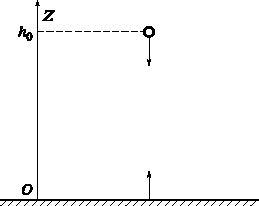
\includegraphics{figure/fig06.01}\vspace{1em}
  \caption{乒乓球的周而复始地上下运动}
  \label{fig:06.01}
\end{wrapfigure}
运转的行星,虽然它的位置及速度时刻在变化着,但总
的来看,它的运动是周而复始地重复。一个钟摆的位置
及速度也在时刻变化着,但总的来看,它的运动也是周
而复始地重复。从高$ h _ { 0 } $处自由落下一个乒乓球,如果球
台的弹性是理想的,则乒乓球会在$ h _ { 0 } $与球台之间弹跳不
止,周而复始地上下运动(图\ref{fig:06.01})。这类的实例,还可举出不少。
它们的共同特点是,在时刻变化的运动状态中,有某种不变的因
素。虽然这些运动能用前面学过的概念加以分析,但我们希望直
接找出描写这种不变性质的物理量。

行星绕太阳运动可以近似为一个匀速圆周运动。它的速度的
方向时刻变化,但是速度的大小$ v $总是不变的,当然$ \dfrac { 1 } { 2 } m v ^ { 2 } $也是
% 167.jpg
\clearpage\noindent
不变的(其中$ m $是行星的质量)。所以,行星运动的不变性质中,至
少有一个可以用下述方程来描写:
\begin{equation}\label{eqn:06.01.01}
  \frac { 1 } { 2 } m v ^ { 2 } = \text{不变量}
\end{equation}
上式左边的量称为行星的动能。因此,在行星运动过程中,可以
说它的动能保持不变,或者说它的动能是守恒的。

对于图6.1的乒乓球的弹跳运动,它的位置与速度大小满足下
列关系
\begin{equation}\label{eqn:06.01.02}
  v = \sqrt { 2 g \left( h _ { 0 } - z \right) }
\end{equation}
此式无论在球的下落还是上弹阶段都是正确的。显然,乒乓球的
动能不再守恒了,因为在运动过程中速度大小时刻在变化。但是
由式\eqref{eqn:06.01.02}可得
\begin{equation}\label{eqn:06.01.03}
  \frac { 1 } { 2 } m v ^ { 2 } + m g z = m g h _ { 0 }
\end{equation}
注意到$ h _ { 0 } , m , g $都是固定的数,这样,乒乓球的弹跳运动的不变
性可以用下述方程来表述:
\begin{equation}\label{eqn:06.01.04}
  \frac { 1 } { 2 } m v ^ { 2 } + m g z = \text{不变量}
\end{equation}
我们称$ mgz $为乒乓球的重力势能。在弹跳过程中,乒乓球的动能
\begin{wrapfigure}[9]{l}{15em}
  \centering
  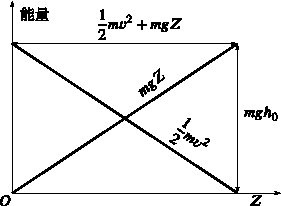
\includegraphics{figure/fig06.02}\vspace{0.6em}
  \caption{落体运动的动能、势能及总能}
  \label{fig:06.02}
\end{wrapfigure}
及重力势能都不是不变的,但是它们的和却保持不变,
或守恒。图6.2上的三条线,分别是乒乓球的动能、重力
势能及它们的总和与高度$ z $的关系。$ z $越大则重力势能
越大,而动能越小;$ z $小时,则相反。我们可以解释为:
在下落过程中,质点的重力势
% 168.jpg
\clearpage
\begin{wrapfigure}[10]{r}{17em}
  \vspace{1em}
  \centering
  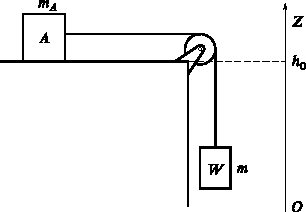
\includegraphics{figure/fig06.03}\vspace{1em}
  \caption{物体在重力作用中的守恒量}
  \label{fig:06.03}
\end{wrapfigure}
\noindent 能渐渐转化为它的动能,而在上弹过程中,
质点的动能渐渐转化为它的重力势能,这两种
形式的能可以相互转化,但总量不变。

对于不是周而复始的运动,也存在类似的
不变量,我们举一个例子来说明。如图6.3,重
物$ W $从$ h _ { 0 } $位置拉着在光滑桌面上的物体$ A $一起运动。如果初始条
件是:$ t = 0 $时,$ W $位于$ h _ { 0 } $,速度为零,则$ W $的位置及速度的解为
\begin{equation*}
  \begin{aligned}
    v & = \frac { m } { m + m _ { A } } g t                                             \\
    z & = h _ { 0 } - \frac { 1 } { 2 } \cdot \frac { m } { m + m _ { A } } g t ^ { 2 }
  \end{aligned}
\end{equation*}
利用上式计算$ W $的动能及重力势能之和:
{\setlength{\mathindent}{2em}
\begin{equation}\label{eqn:06.01.05}
  \begin{aligned}
     & \quad \, \frac { 1 } { 2 } m v ^ { 2 } + m g z                                                                                                                                                    \\
     & = \frac { 1 } { 2 } m \left( \frac { m } { m + m _ { A } } \right) ^ { 2 } g ^ { 2 } t ^ { 2 } + m g \left( h _ { 0 } - \frac { 1 } { 2 } \cdot \frac { m } { m + m _ { A } } g t ^ { 2 } \right) \\
     & = m g h _ { 0 } - \frac { 1 } { 2 } m _ { A } \left( \frac { m } { m + m _ { A } } \right) ^ { 2 } g ^ { 2 } t ^ { 2 }
  \end{aligned}
\end{equation}}
由于结果含$ t $,表示$ W $的动能及重力势能之和不再守恒了。但是,
我们注意到,这个运动所产生的后果,不仅引起了$ W $的运动,而
且还引起了$ A $的运动。当$ W $具有速度$ v $时,$ A $也具有速度$ v $,故$ A $具有有动能
$ \dfrac { 1 } { 2 } m _ { A } v ^ { 2 } = \dfrac { 1 } { 2 } m _ { A } \left( \dfrac { m } { m + m _ { A } } \right) ^ { 2 } g ^ { 2 } t ^ { 2 } $
,这样,式\eqref{eqn:06.01.05}
% 169.jpg
可改写为
\begin{equation*}
  \frac { 1 } { 2 } m v ^ { 2 } + m g z + \frac { 1 } { 2 } m _ { A } v ^ { 2 } = m g h _ { 0 }
\end{equation*}
这个结果告诉我们,在运动过程中,物体$ W $与物体$ A $的能量都在
变化着,但二者的动能与重力势能之和不变化,是守恒的,即
\begin{equation}\label{eqn:06.01.06}
  \frac { 1 } { 2 } m v ^ { 2 } + m g z + \frac { 1 } { 2 } m _ { A } v ^ { 2 } = \text{不变量}
\end{equation}

一般地说,对每个质量为$ m $的质点,我们可以定义它的动能
为
\begin{equation*}
  T = \frac { 1 } { 2 } m v ^ { 2 }
\end{equation*}
在重力作用下的质量为$ m $的质点,可以定义它的重力势能为
\begin{equation*}
  V = m g z
\end{equation*}
动能和势能是描写机械运动的重要的物理量,它们的重要之处就
在于由这些量常常能构成一些不变量。在运动过程中,物体的动
能和势能一般会发生变化,一物体的动能和势能之间会发生转化,
物体之间的动能和势能也会发生转化。但对有些机械运动来说,
参与运动的各物体的动能$ T $及势能$ V $之和保持不变。物体体系的
动能和势能总称为机械能。所以,这条规律又称为机械能守恒定
律,可以表示成
\begin{equation}\label{eqn:06.01.07}
  E = T + V = \text{不变量}
\end{equation}
其中$ E $表示体系的能量,它的量纲是$ [ E ] = [ m ][ v ^ { 2 } ] = M L ^ { 2 } T ^ { - 2 } $,
在MKS制(或SI)中,它的单位是焦耳,一个焦耳的能等于质量1
千克的物体以速度1米/秒运动时所具有的动能。

机械能守恒定律\lhbrak 式\eqref{eqn:06.01.07}\rhbrak ,对于许多运动并不成立。滑行
着的自行车会慢慢停下来,它的机械能慢慢在减小。可以说凡有
摩擦力参与的运动,其机械能一般是不守恒的。

那么,这些机械能是否不留痕迹地消失了?不是的,摩擦的
% 170.jpg
结果使接触面处的温度升高了。如自行车机械能消失了,路面与
车轮接触处温升的热能却作为“痕迹”留下了。温度是物质中分
子无规运动的表现。分子无规运动的动能愈高,物质的温度也愈
高。所以,自行车的机械能并没有消失,而是转化成分子无规运
动的能量,即物体的内能。这时机械能守恒定律\lhbrak 式\eqref{eqn:06.01.07}\rhbrak 不再
成立。但是,如果考虑到机械能转化成内能,可以把式\eqref{eqn:06.01.07}推
广成为
\begin{equation*}
  T + V + \text{内能} = \text{不变量}
\end{equation*}
这就是更一般的能量守恒定律。

物理现象中,除了机械能,内能之外,还有许多其他形式的
能量,诸如与原子间作用相联系的化学能,与电磁作用相联系的
电磁能、辐射能,与原子核间作用联系的核能等等。在一般的运
动过程中,个别形式的能量是变化的,不同形式的能量之间可以
相互转化,但如果我们计及所有形式的能量,则对任何运动过
程,能量的总和是不变的、守恒的。这个最一般的能量守恒定律,
是一条非常普适的物理规律,它被现今的所有实验所证实。

这一节的分析告诉我们,寻找运动中的不变量或守恒量是很
有用的一种方法。因为,不变量往往能更清楚地描写运动,标志
运动的特征;而且,守恒的物理量往往有更大的适用范围,象能
量这一概念,适用于牛顿力学所讨论的机械运动,同样又适用于
牛顿力学所不能讨论的其他运动形态。
